\documentclass[compress,trans,9pt]{beamer}
%\documentclass[compress,9pt,usenames,dvipsnames]{beamer}
% \usepackage[utf8]{inputenc}
% \includeonlyframes{current}
\setbeamercovered{dynamic}
\usepackage{etex}
\usepackage{graphicx,url,psfrag}
\usepackage{tikz}
\usetikzlibrary{decorations.pathreplacing,calc,decorations.fractals,through,shapes,patterns,arrows.meta,decorations.pathreplacing,arrows,shapes,}
\usepackage{tikzpeople}
% \usepackage[center]{subfigure}
\usepackage{enumerate}
\usepackage[makeroom]{cancel}
\usepackage{mathtools}
\usepackage{graphbox}
\usepackage{amssymb}
\usepackage{comment}
\excludecomment{codes}
% \usepackage{movie15}
% \usepackage[showframe]{geometry}
% \usepackage{enumitem}

%
% for warning sign
%
\usepackage{pgfplots}
\usepackage{stackengine}
\usepackage{scalerel}
\usepackage{xcolor}
\usepackage{dbt}
\newcommand\dangersign[1][2ex]{%
  \renewcommand\stacktype{L}%
  \scaleto{\stackon[1.3pt]{\color{red}$\triangle$}{\tiny !}}{#1}%
}
% %  The following is to show codes:
\usepackage{listings}
% \usepackage{color}

\usepackage{pifont}% http://ctan.org/pkg/pifont
\newcommand{\cmark}{\ding{51}}%
\newcommand{\xmark}{\ding{55}}%

\definecolor{dkgreen}{rgb}{0,0.6,0}
\definecolor{gray}{rgb}{0.5,0.5,0.5}
\definecolor{mauve}{rgb}{0.58,0,0.82}

\lstset{frame=tb,
  language=Java,
  aboveskip=3mm,
  belowskip=3mm,
  showstringspaces=false,
  columns=flexible,
  basicstyle={\small\ttfamily},
  numbers=none,
  numberstyle=\tiny\color{gray},
  keywordstyle=\color{blue},
  commentstyle=\color{dkgreen},
  stringstyle=\color{mauve},
  breaklines=true,
  breakatwhitespace=true,
  tabsize=3
}
\lstset{language=Python}

\lstset{ %
  language=Python,                     % the language of the code
  basicstyle=\footnotesize,       % the size of the fonts that are used for the code
  numbers=left,                   % where to put the line-numbers
  numberstyle=\tiny\color{gray},  % the style that is used for the line-numbers
  stepnumber=1,                   % the step between two line-numbers. If it's 1, each line
                                  % will be numbered
  numbersep=5pt,                  % how far the line-numbers are from the code
  backgroundcolor=\color{black},  % choose the background color. You must add \usepackage{color}
  showspaces=false,               % show spaces adding particular underscores
  showstringspaces=false,         % underline spaces within strings
  showtabs=false,                 % show tabs within strings adding particular underscores
  frame=single,                   % adds a frame around the code
  rulecolor=\color{black},        % if not set, the frame-color may be changed on line-breaks within not-black text (e.g. commens (green here))
  tabsize=2,                      % sets default tabsize to 2 spaces
  captionpos=b,                   % sets the caption-position to bottom
  breaklines=true,                % sets automatic line breaking
  breakatwhitespace=false,        % sets if automatic breaks should only happen at whitespace
  title=\lstname,                 % show the filename of files included with \lstinputlisting;
                                  % also try caption instead of title
  keywordstyle=\color{blue},      % keyword style
  commentstyle=\color{dkgreen},   % comment style
  stringstyle=\color{mauve},      % string literal style
  escapeinside={\%*}{*)},         % if you want to add a comment within your code
  morekeywords={*,...}            % if you want to add more keywords to the set
}
% \usepackage[usenames,dvipsnames]{color}
% \lstset{
%   language=R,                     % the language of the code
%   basicstyle=\tiny\ttfamily, % the size of the fonts that are used for the code
%   numbers=left,                   % where to put the line-numbers
%   numberstyle=\tiny\color{Blue},  % the style that is used for the line-numbers
%   stepnumber=1,                   % the step between two line-numbers. If it is 1, each line
%                                   % will be numbered
%   numbersep=5pt,                  % how far the line-numbers are from the code
%   backgroundcolor=\color{white},  % choose the background color. You must add \usepackage{color}
%   showspaces=false,               % show spaces adding particular underscores
%   showstringspaces=false,         % underline spaces within strings
%   showtabs=false,                 % show tabs within strings adding particular underscores
%   frame=single,                   % adds a frame around the code
%   rulecolor=\color{black},        % if not set, the frame-color may be changed on line-breaks within not-black text (e.g. commens (green here))
%   tabsize=2,                      % sets default tabsize to 2 spaces
%   captionpos=b,                   % sets the caption-position to bottom
%   breaklines=true,                % sets automatic line breaking
%   breakatwhitespace=false,        % sets if automatic breaks should only happen at whitespace
%   keywordstyle=\color{RoyalBlue},      % keyword style
%   commentstyle=\color{YellowGreen},   % comment style
%   stringstyle=\color{ForestGreen}      % string literal style
% }

% \usepackage[dvipsnames]{xcolor}
% \newcommand{\Cross}{\mathbin{\tikz [x=1.4ex,y=1.4ex,line width=.2ex] \draw (0,0) -- (1,1) (0,1) -- (1,0);}}%
\newcommand{\Crossme}[1]{\!\!
\tikz [black,x=1.1em,y=1.1em,line width=.4ex]
\draw (-0.5,-0.5) -- (0,0) node {\footnotesize #1} -- (0.5,0.5) (0.5,-0.5) -- (-0.5,0.5);}%
\newcommand{\Checkme}[1]{\!\!
\tikz [x=1.1em,y=1.1em,line width=.4ex]
\draw [black] (0,0.7) -- (0.3,0) --(0.9,1.0) (0.5,0.5) node {\footnotesize #1};}
% \beamerdefaultoverlayspecification{<+-| alert@+>} %(this will show line by line)
\beamerdefaultoverlayspecification{<+->} %(this will show line by

% \usepackage{natbib}
% \input{../myMathSymbols.tex}
% \newcommand{\tlMr}[4]{\:{}^{\hspace{0.2em}#1}_{#2} \hspace{-0.1em}#3_{#4}}

% Smiley face\Smiley{} \Frowny{}
\usepackage{marvosym}
% -------------------------------------------------
%  Set directory for figs
% -------------------------------------------------
\usepackage{grffile}
\graphicspath{{Codes/}}
% -------------------------------------------------
%  Define colors
% -------------------------------------------------
\def\refcolor{cyan}
\def\excolor{brown}
% \usepackage{color}
% \usepackage[dvipsnames]{xcolor}


% % % Define danger sign
\newcommand*{\TakeFourierOrnament}[1]{{%
\fontencoding{U}\fontfamily{futs}\selectfont\char#1}}
\newcommand*{\danger}{\TakeFourierOrnament{66}}


% -------------------------------------------------
%  Define short-hand symbols.
% -------------------------------------------------
\newcommand{\B}{\textbf{B}}
\newcommand{\PP}{\mathbb{P}}
\newcommand{\E}{\mathbb{E}}
\newcommand{\D}{\mathbb{D}}
\newcommand{\W}{\dot{W}}
\newcommand{\ud}{\ensuremath{\mathrm{d}}}
\newcommand{\Ceil}[1]{\left\lceil #1 \right\rceil}
\newcommand{\Floor}[1]{\left\lfloor #1 \right\rfloor}
\newcommand{\sgn}{\text{sgn}}
\newcommand{\Lad}{\text{L}_{\text{ad}}^2}
\newcommand{\SI}[1]{\mathcal{I}\left[#1 \right]}
\newcommand{\SIB}[2]{\mathcal{I}_{#2}\left[#1 \right]}
\newcommand{\Indt}[1]{1_{\left\{#1 \right\}}}
\newcommand{\LadInPrd}[1]{\left\langle #1 \right\rangle_{\text{L}_\text{ad}^2}}
\newcommand{\LadNorm}[1]{\left|\left|  #1 \right|\right|_{\text{L}_\text{ad}^2}}
\newcommand{\Norm}[1]{\left|\left|  #1   \right|\right|}
\newcommand{\Ito}{It\^{o} }
\newcommand{\Itos}{It\^{o}'s }
\newcommand{\spt}[1]{\text{supp}\left(#1\right)}
\newcommand{\InPrd}[1]{\left\langle #1 \right\rangle}
\newcommand{\mr}{\textbf{r}}
\newcommand{\Ei}{\text{Ei}}
\newcommand{\arctanh}{\operatorname{arctanh}}
\newcommand{\ind}[1]{\mathbb{I}_{\left\{ {#1} \right\} }}
\newcommand{\Var}{\text{Var}}
\newcommand{\Cov}{\text{Cov}}
\newcommand{\Corr}{\text{Corr}}

\newcommand{\baseurl}[1]{\footnotesize\url{http://math.emory.edu/~lchen41/teaching/2020_Spring/#1}}


\newcommand*\mystrut[1]{\vrule width0pt height0pt depth#1\relax} % adding vertical space

\DeclareMathOperator{\esssup}{\ensuremath{ess\,sup}}

\newcommand{\steps}[1]{\vskip 0.3cm \textbf{#1}}
\newcommand{\calB}{\mathcal{B}}
\newcommand{\calC}{\mathcal{C}}
\newcommand{\calD}{\mathcal{D}}
\newcommand{\calE}{\mathcal{E}}
\newcommand{\calF}{\mathcal{F}}
\newcommand{\calG}{\mathcal{G}}
\newcommand{\calK}{\mathcal{K}}
\newcommand{\calH}{\mathcal{H}}
\newcommand{\calI}{\mathcal{I}}
\newcommand{\calL}{\mathcal{L}}
\newcommand{\calM}{\mathcal{M}}
\newcommand{\calN}{\mathcal{N}}
\newcommand{\calO}{\mathcal{O}}
\newcommand{\calT}{\mathcal{T}}
\newcommand{\calP}{\mathcal{P}}
\newcommand{\calR}{\mathcal{R}}
\newcommand{\calS}{\mathcal{S}}
\newcommand{\calV}{\mathcal{V}}
\newcommand{\bbC}{\mathbb{C}}
\newcommand{\bbN}{\mathbb{N}}
\newcommand{\bbP}{\mathbb{P}}
\newcommand{\bbZ}{\mathbb{Z}}
\newcommand{\myVec}[1]{\overrightarrow{#1}}
\newcommand{\sincos}{\begin{array}{c} \cos \\ \sin \end{array}\!\!}
\newcommand{\CvBc}[1]{\left\{\:#1\:\right\}}
\newcommand*{\one}{{{\rm 1\mkern-1.5mu}\!{\rm I}}}

\newcommand{\OneFrame}[1]{
\begin{enumerate}\item[#1] \phantom{av} \\[20em]\vfill\phantom{av}\myEnd\end{enumerate}}

\newcommand{\bH}{\ensuremath{\mathrm{H}}}
\newcommand{\Ai}{\ensuremath{\mathrm{Ai}}}

\newcommand{\R}{\mathbb{R}}
\newcommand{\myEnd}{\hfill$\square$}
\newcommand{\ds}{\displaystyle}
\newcommand{\Shi}{\text{Shi}}
\newcommand{\Chi}{\text{Chi}}
\newcommand{\Erf}{\ensuremath{\mathrm{erf}}}
\newcommand{\Erfc}{\ensuremath{\mathrm{erfc}}}
\newcommand{\He}{\ensuremath{\mathrm{He}}}
\newcommand{\Res}{\ensuremath{\mathrm{Res}}}

\newcommand{\mySeparateLine}{\begin{center}
 \makebox[\linewidth]{\rule{0.6\paperwidth}{0.4pt}}
\end{center}}

\theoremstyle{definition}
% \newtheorem{definition}[theorem]{Definition}
% \newtheorem{hypothesis}[theorem]{Hypothesis}
\newtheorem{assumption}[theorem]{Assumption}

\theoremstyle{plain}
% \newtheorem{theorem}{Theorem}
% \newtheorem{corollary}[theorem]{Corollary}
% \newtheorem{lemma}[theorem]{Lemma}
\newtheorem{proposition}[theorem]{Proposition}

\mode<presentation>
{
%      \usetheme{Warsaw}
%     \usetheme{JuanLesPins}
%  \usetheme{Hannover}
%  \usetheme{Montpellier}
   \useoutertheme{default}
  % or ...

  \setbeamercovered{transparent}
  % or whatever (possibly just delete it)
 \setbeamertemplate{frametitle}{
  \begin{centering}
    \color{blue}
    {\insertframetitle}
    \par
  \end{centering}
  }
}
\usefoottemplate{\hfill \insertframenumber{}}
% \inserttotalframenumber

\usepackage[english]{babel}
% or whatever

% \usepackage[latin1]{inputenc}
% or whatever

\usepackage{times}
\usepackage[T1]{fontenc}
% Or whatever. Note that the encoding and the font should match. If T1
% does not look nice, try deleting the line with the fontenc.

% \DeclareMathOperator{\Lip}{Lip}
\DeclareMathOperator{\lip}{l}
% \DeclareMathOperator{\Vip}{\overline{v}}
% \DeclareMathOperator{\vip}{\underline{v}}
% \DeclareMathOperator{\vv}{v}
% \DeclareMathOperator{\BC}{BC}
% \DeclareMathOperator{\CH}{CD}

\usepackage{pgfpages}
% \setbeameroption{show notes}
% \setbeamertemplate{note page}[plain]
% \setbeameroption{second mode text on second screen=right}
% \setbeameroption{show notes on second screen=right}
%

% Delete this, if you do not want the table of contents to pop up at
% the beginning of each subsection:
% \AtBeginSubsection[]
% {
%   \begin{frame}<beamer>{Outline}
%     \tableofcontents[currentsection,currentsubsection]
%   \end{frame}
% }

% If you wish to uncover everything in a step-wise fashion, uncomment
% the following command:
% \beamerdefaultoverlayspecification{<+->}

% % % % % % % % % % % % % % % % % % %
%  Define a block
% % % % % % % % % % % % % % % % % % %
\newenvironment<>{problock}[1]{%
  \begin{actionenv}#2%
      \def\insertblocktitle{#1}%
      \par%
      \mode<presentation>{%
        \setbeamercolor{block title}{fg=white,bg=olive!95!black}
       \setbeamercolor{block body}{fg=black,bg=olive!25!white}
       \setbeamercolor{itemize item}{fg=white!20!white}
       \setbeamertemplate{itemize item}[triangle]
     }%
      \usebeamertemplate{block begin}}
    {\par\usebeamertemplate{block end}\end{actionenv}}

\newenvironment<>{assblock}[1]{%
  \begin{actionenv}#2%
      \def\insertblocktitle{#1}%
      \par%
      \mode<presentation>{%
        \setbeamercolor{block title}{fg=white,bg=green!50!black}
       \setbeamercolor{block body}{fg=black,bg=green!10}
       \setbeamercolor{itemize item}{fg=green!80!black}
       \setbeamertemplate{itemize item}[triangle]
     }%
      \usebeamertemplate{block begin}}
    {\par\usebeamertemplate{block end}\end{actionenv}}


% \newtheorem{proofnoend}{Proof.}
% \AtBeginEnvironment{proofnoend}{%
%   \setbeamercolor{block title}{use=example text,fg=lgtblue,bg=background}
%   % \setbeamercolor{block body}{parent=normal text,use=block title example,fg=yellow}
% }

% Define some colors
\definecolor{white}{HTML}{FFFFFF}              % #FFFFFF
\definecolor{pink}{HTML}{FB73BE}               % #FB73BE
\definecolor{coral}{HTML}{FF8D71}              % #FF8D71
\definecolor{yellow}{HTML}{FFE066}             % #FFE066
\definecolor{teal}{HTML}{59F3CE}               % #59F3CE
\definecolor{lgtblue}{HTML}{65D0FA} 	       % #65D0FA
\definecolor{blue}{HTML}{4984F2}               % #4984F2
\definecolor{purple}{HTML}{A87DFF}             % #A87DFF
\definecolor{red}{HTML}{FF3d30}                % #FF3d30
% \definecolor{magenta}{HTML}{FF80FF}                % #FF3d30
\definecolor{green}{HTML}{BBFFB9}              % #BBFFB9
% \definecolor{green}{HTML}{59F3CE}              % #BBFFB9
\setbeamercolor{alerted text}{fg=red}
% \setbeamercolor{block title}{bg=background,fg=lgtblue}

\setbeamercolor{section in toc}{fg=yellow}
\setbeamercolor{subsection in toc}{fg=red}

% \newtheorem{myexample}{\it Example}[section]
\newcounter{myexample}[section]
\resetcounteronoverlays{myexample}
\newenvironment{myexample}[1][]{\refstepcounter{myexample}\par\medskip
\noindent \textbf{\textcolor{green}{Example~\mySecNum-\themyexample~#1}} \rmfamily}{\medskip}

\newcounter{mydefinition}[section]
\resetcounteronoverlays{mydefinition}
\newenvironment{mydefinition}[1][]{\refstepcounter{mydefinition}\par\medskip
\noindent \textbf{\textcolor{yellow}{Definition~\mySecNum-\themydefinition~#1}} \rmfamily}{\medskip}

% \NewCommandCopy{\oldref}{\ref}
% \let\oldref\ref
\newcommand{\myref}[1]{\mySecNum-\ref{#1}}

\newcounter{remark}[section]
\resetcounteronoverlays{remark}
\newenvironment{remark}[1][]{\refstepcounter{remark}\par\medskip
\noindent \textbf{\textcolor{blue}{Remark~\mySecNum-\theremark~#1}} \rmfamily}{\medskip}

\newcounter{mythm}[section]
\resetcounteronoverlays{mythm}
\newenvironment{mythm}[1][]{\refstepcounter{mythm}\par\medskip
\noindent \textbf{\textcolor{lgtblue}{Theorem~\mySecNum-\themythm~#1}} \rmfamily}{\medskip}

\newenvironment{mycor}[1][]{\refstepcounter{mythm}\par\medskip
\noindent \textbf{\textcolor{lgtblue}{Corollary~\mySecNum-\themythm~#1}} \rmfamily}{\medskip}

% \newtheorem{solution}{\textcolor{purple}{Solution}}
\newenvironment{mysol}[1][]{\par\medskip
\noindent \textbf{\textcolor{purple}{Solution#1.~}} \rmfamily}{\medskip}

\newenvironment{myproof}[1][]{\par\medskip
\noindent \textbf{\textcolor{purple}{Proof#1.~}} \rmfamily}{\medskip}

\long\def\script#1{}

% \numberwithin{equation}{section}

% If you have a file called "university-logo-filename.xxx", where xxx
% is a graphic format that can be processed by latex or pdflatex,
% resp., then you can add a logo as follows:

% \pgfdeclareimage[height=1cm]{Emory}{figs/Emory.png}


\title % (optional, use only with long paper titles)
{
  Financial Mathematics \\
  \bigskip
  \small MATH 5870/6870\footnote{\textcolor{gray}{Based on Robert L. McDonald's {\it Derivatives Markets}, 3rd Ed, Pearson, 2013.}}\\
  Fall 2021
}

% \subtitle
% {Research Plan} % (optional)

\author{Le Chen\\[1em]
  {\small\textcolor{gray}{\url{lzc0090@auburn.edu}}}
}


\institute[Auburn University]
{
% \pgfuseimage{Emory}\\[3em]
% {\small Auburn University}\\[1em]
% {\small Auburn AL}\\[3em]
\textcolor{gray}{Last updated on } \\[1em]
\textcolor{gray}{\today}
 \vspace{8em}
}
% - Use the \inst command only if there are several affiliations.
% - Keep it simple, no one is interested in your street address.

\date[Auburn]{Auburn University\\ \textcolor{gray}{Auburn AL}}
% \date{}

% \subject{}



\begin{document}
\begin{frame}[noframenumbering]
  \titlepage
\end{frame}
\newcommand{\myChapter}{Chapter 2. An Introduction to Forwards and Options}
\newcommand{\mySection}[1]{
  \section{\S\: #1}
  \begin{frame}{\myChapter}\tableofcontents\end{frame}
  \begin{frame}{\myChapter}\tableofcontents[currentsection]\end{frame}
  }
\begin{frame}
\begin{center}
\huge
\myChapter
\end{center}
\end{frame}
\def\mySecNum{2.1}
\mySection{\mySecNum~Forward contracts}
%-------------- start slide -------------------------------%{{{ 1
\begin{frame}[fragile,t]
	\begin{mydefinition}
		\textcolor{magenta}{Forward contract} is a binding agreement (obligation) to buy or sell an
		underlying asset in the future, at a price set today.  The time at which the contract settles is
		called the \textcolor{magenta}{expiration date}.  A forward contract specifies
		\begin{itemize}
			\item The features and quantity of the asset to be delivered.
			\item The delivery logistics, such as time, date, and place.
			\item The price the buyer will pay at the time of delivery.
		\end{itemize}
	\end{mydefinition}
	\bigskip
	\begin{remark}
		\begin{enumerate}
			\item \textcolor{magenta}{Futures contracts} are the same as forwards in principle except for
				some institutional and pricing differences. We will study future contracts in Chapter 5.
			\item A forward contract requires no initial payment or \textcolor{magenta}{premium}.
		\end{enumerate}
	\end{remark}
\end{frame}
%-------------- end slide -------------------------------%}}}
%-------------- start slide -------------------------------%{{{ 1
\begin{frame}[fragile,t]
	\begin{center}
		\textcolor{green}{Long} = buy \qquad \textcolor{red}{short} = sell
	\end{center}

	\bigskip
	\begin{mydefinition}
		\textcolor{magenta}{Payoff for a contract} is its value at expiration. In particular, for
		forward contracts,
		\bigskip
		\begin{center}
			Payoff for \textcolor{green}{Long} forward = Spot price at expiration $-$ Forward price \\ \bigskip
			Payoff for \textcolor{red}{Short} forward = Forward price $-$ Spot price at expiration
		\end{center}
	\end{mydefinition}
	\vfill

	\begin{remark}
		Payoff and \textcolor{magenta}{profit (net payoff)} are the same for forward contracts because
		there is no initial payment -- \textcolor{cyan}{premium}.
	\end{remark}
\end{frame}
%-------------- end slide -------------------------------%}}}
%-------------- start slide -------------------------------%{{{ 1
\begin{frame}[fragile,t]
	\begin{myexample}
	  S\&R (special and rich) index:
		\begin{center}
			Today: Spot price = \$1,000\\
			6-month forward price = \$1,020 \\
			In six months at contract expiration: Spot price = \$1,050.
		\end{center}
		What are the payoff of long/short forward?
	\end{myexample}
	\bigskip
	\pause
	\begin{mysol}
		\begin{center}
		Long position payoff $=\$1,050-\$1,020 = \$30$, \\ \bigskip
		Short position payoff $= \$1,020-\$1,050 = (\$30)$.
		\end{center}
		\myEnd
	\end{mysol}
\end{frame}
%-------------- end slide -------------------------------%}}}
%-------------- start slide -------------------------------%{{{ 1
\begin{frame}[fragile,t]
	% \frametitle{Payoff diagram for forwards}
\begin{center}
	Payoff diagram for a forward price = \$1,020 \\
	\bigskip

	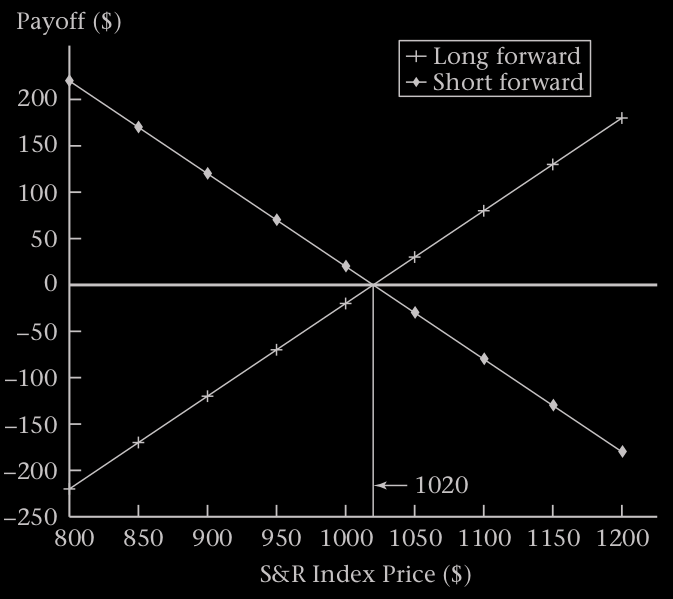
\includegraphics[scale=0.2]{figs/Figure-2-2.png}
\end{center}
\end{frame}
%-------------- end slide -------------------------------%}}}
%-------------- start slide -------------------------------%{{{ 1
\begin{frame}[fragile,t]
	\frametitle{Forward versus outright purchase}
	We will see this through the following example:

	\begin{myexample}
		S\&R 6-month forward contract with a zero-coupon bound (e.g., Treasury bills).
		The 6-month interest rate is $2\%$. Spot price today $= \$1,000$.
	\end{myexample}
\end{frame}
%-------------- end slide -------------------------------%}}}
%-------------- start slide -------------------------------%{{{ 1
\begin{frame}[fragile,t]
	\begin{center}
		\$1,000 today is worth $\$1,000 \times 1.02 = \$1,020$ in 6 months.

	\bigskip
	\mySeparateLine
	\bigskip

	\textcolor{magenta}{Outright purchase}\footnote{It is also called \textcolor{magenta}{long physical index}.} is equivalent to
	\textcolor{cyan}{forward + bond}\footnote{Invest \$1,000 to bond for 6 month and enter long
	position of forward contract at the same time.}\\

	\bigskip
	because\\
	\bigskip

	\begin{align*}
		\text{Payoff of \textcolor{cyan}{forward+bond}} & = \underbrace{\text{Spot price at expiration} - \$1,020}_{\text{Forward payoff}} + \underbrace{\$1,020}_{\text{Bound payoff}} \\
                                                    & = \text{Spot price at expiration}                                                                                             \\
																										& = \text{Payoff of \textcolor{magenta}{outright purchase}}
	\end{align*}
	% \bigskip
  %
	% 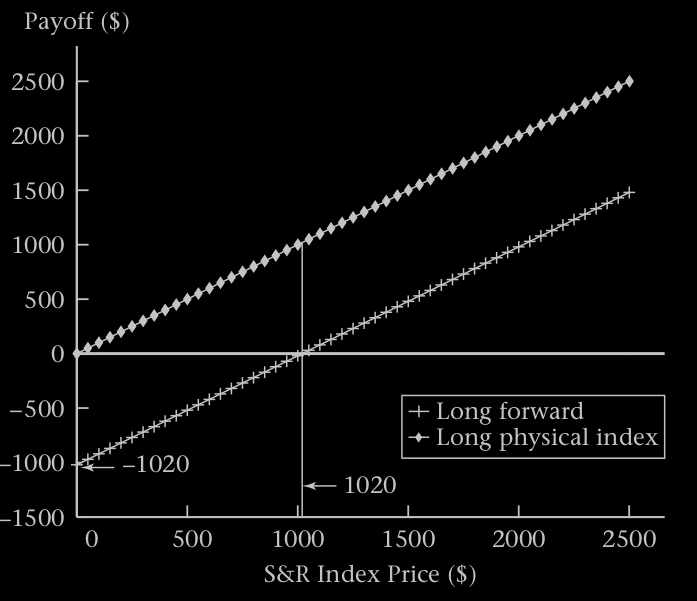
\includegraphics[scale=0.2]{figs/Figure-2-3.png}
	% 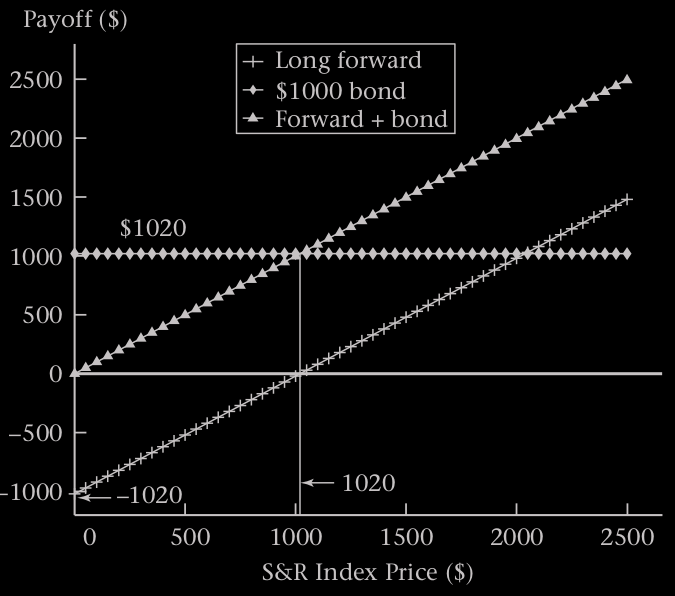
\includegraphics[scale=0.2]{figs/Figure-2-4.png}

	% \bigskip
	\end{center}
\end{frame}
%-------------- end slide -------------------------------%}}}
%-------------- start slide -------------------------------%{{{ 1
\begin{frame}[fragile,t]
	\begin{center}
		\$1,000 today is worth $\$1,000 \times 1.02 = \$1,020$ in 6 months.

	\bigskip
	\mySeparateLine
	\bigskip

	\textcolor{magenta}{Long forward} is equivalent to
	\textcolor{cyan}{borrow-to-buy}\footnote{Borrow money (\$1,000) to outright buy physical index and at expiration
	pay back the money (\$1,020).}

	\bigskip
	because\\
	\bigskip


	\begin{align*}
		\text{Payoff of \textcolor{cyan}{borrow-to-buy}} & = \underbrace{\text{Spot price at expiration}}_{\text{Payoff for outright buy}} - \underbrace{\$1,020}_{\text{Return borrowed money}} \\[1em]
																										 & = \text{Payoff of \textcolor{magenta}{long forward}}.
	\end{align*}

	% \bigskip
  %
	% 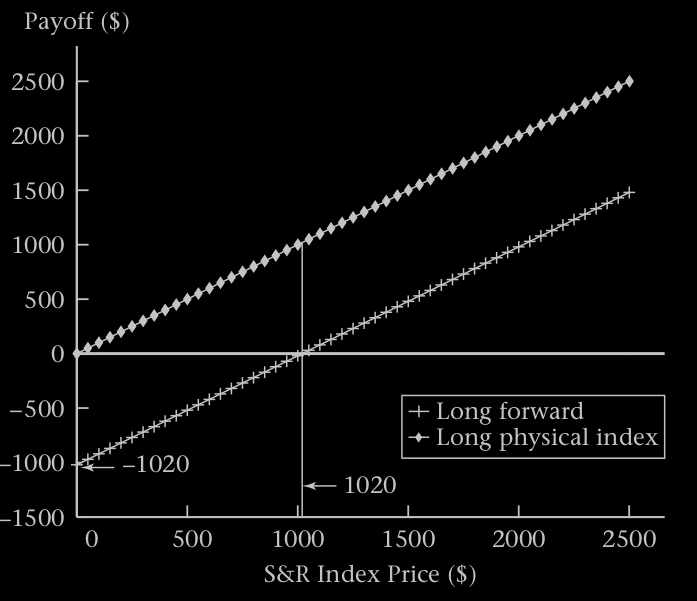
\includegraphics[scale=0.2]{figs/Figure-2-3.png}
	% 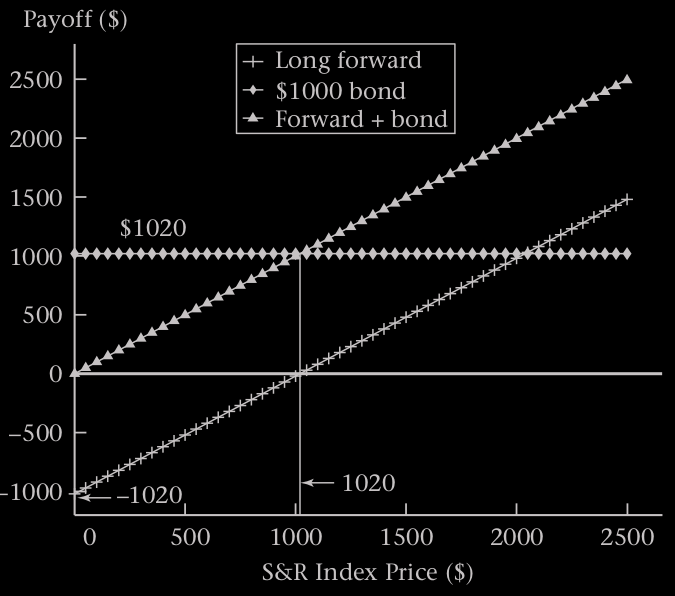
\includegraphics[scale=0.2]{figs/Figure-2-4.png}

	% \bigskip
	\end{center}
\end{frame}
%-------------- end slide -------------------------------%}}}
%-------------- start slide -------------------------------%{{{ 1
\begin{frame}[fragile]
\begin{center}
	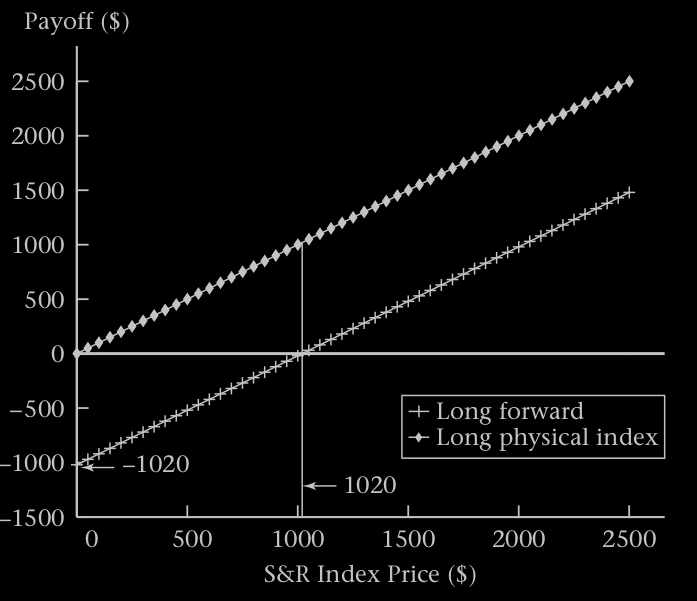
\includegraphics[scale=0.2]{figs/Figure-2-3.png}
	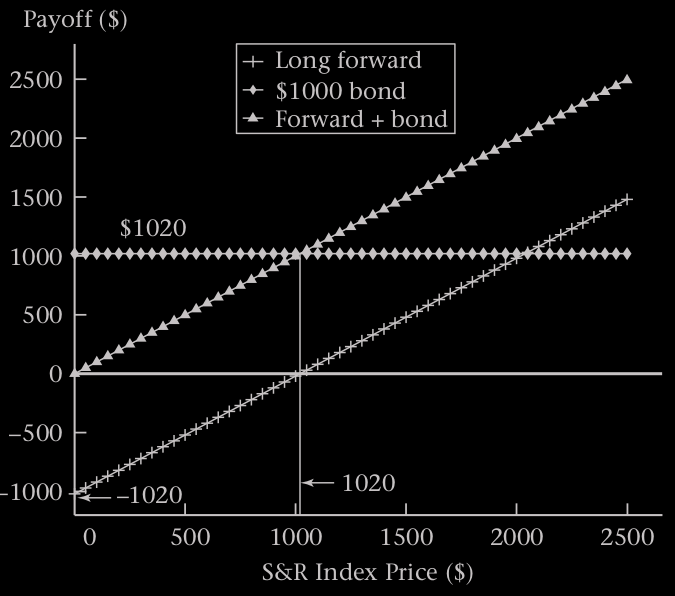
\includegraphics[scale=0.2]{figs/Figure-2-4.png}
\end{center}
\end{frame}
%-------------- end slide -------------------------------%}}}
%-------------- start slide -------------------------------%{{{ 1
\begin{frame}[fragile,t]
	\frametitle{Cash settlement versus physical delivery \\[0.5em]  -- Type of settlement}

	\begin{itemize}
		\item Cash settlement: less costly and more practical
		\item Physical delivery: often avoided due to significant costs
	\end{itemize}
	\bigskip
	\bigskip
	\pause

	\begin{myexample}
		Consider the S\&R index with the forward price \$1,020.\\
		\bigskip

		\begin{itemize}
			\item Suppose that the S\&R index at expiration is \$1,040.
			\item The long position has a payoff of \$20.
			\item Similarly, the short position loses \$20.
		\end{itemize}
		\pause With \textcolor{cyan}{cash settlement}, the short simply pays \$20 to the long, with
		\textcolor{cyan}{no transfer of the physical asset}, and hence \textcolor{cyan}{no transaction
		costs}.  It is as if the long paid \$1,020, acquired the index worth \$1,040, and then
		immediately sold it with no transaction costs.

		\pause
		\mySeparateLine
		\bigskip

		\begin{itemize}
			\item Suppose that the S\&R index price at expiration had instead been \$960.
			\item The long position would have a payoff of $-\$60$.
			\item The short would have a payoff of \$60.
		\end{itemize}
		\pause
		\textcolor{cyan}{Cash settlement} in this case entails the long paying \$60 to the short.
	\end{myexample}
\end{frame}
%-------------- end slide -------------------------------%}}}
%-------------- start slide -------------------------------%{{{ 1
\begin{frame}[fragile,t]
	\frametitle{Credit risk}

	All derivatives contracts have \textcolor{magenta}{credit risk}, which is the possibility that the
	counterparty who owes money fails to make a payment.  \bigskip

	\begin{itemize}
		\item Major issue for \textcolor{magenta}{over-the-counter (OTC) contracts}\\[1em]
			\textcolor{cyan}{Credit check} \\
			\textcolor{cyan}{Credit protections} such as collateral and bank letter of credit
		\bigskip
	\item Less severe for \textcolor{magenta}{exchange-traded contracts}\\[1em]
		Exchange guarantees transactions, requires collateral
	\end{itemize}
\end{frame}
%-------------- end slide -------------------------------%}}}

\def\mySecNum{2.2}
\mySection{\mySecNum~Call options}
%-------------- start slide -------------------------------%{{{ 1
\begin{frame}[fragile,t]
\begin{center}
	Can one modify the forward contract so that\\
	the buyer can walk away from the deal at expiration?
\end{center}
\bigskip
\mySeparateLine
\bigskip

\begin{mydefinition}
	A \textcolor{magenta}{call option} is a contract where the buyer has the right to buy, but not the obligation to buy.
\end{mydefinition}
\bigskip

\end{frame}
%-------------- end slide -------------------------------%}}}
%-------------- start slide -------------------------------%{{{ 1
\begin{frame}[fragile,t]
	\begin{myexample}
		S\&R index: Buyers' perspective
		\begin{itemize}
			\item Today: call buyer acquires the right to pay \$1,020 in six months for the index, but is not obligated to do so
			\item In six months at contract expiration: \\
				if the spot price is \$1,100, call buyer’s payoff $=\$1,100-\$1,020=\$80$\\
				if the spot price is \$900, call buyer walks away, buyer’s payoff = \$0.
		\end{itemize}
	\end{myexample}

	\pause
	\bigskip
	\mySeparateLine
	\bigskip

	\begin{myexample}
		S\&R index: Sellers' perspective
		\begin{itemize}
			\item Today: call seller is obligated to sell the index for \$1,020 in six months, if asked to do so
			\item In six months at contract expiration: \\
				if the spot price is \$1,100, call seller’s payoff $=\$1,020-\$1,100=-\$80$\\
				if the spot price is \$900, call buyer walks away, seller’s payoff = \$0.
		\end{itemize}
	\end{myexample}
\end{frame}
%-------------- end slide -------------------------------%}}}
%-------------- start slide -------------------------------%{{{ 1
\begin{frame}[fragile]
\begin{center}
	\begin{minipage}{0.8\textwidth}
		\begin{itemize}
			\item[\textcolor{magenta}{Buyer}] preserves the upside potential, while at the same time eliminates the unpleasant
				downside.
				\bigskip

				\begin{align*}
					\text{However}
				\end{align*}
				\bigskip

			\item[\textcolor{cyan}{Seller}] has to be compensated by a initial premium for being at a disadvantage at
				expiration.
		\end{itemize}
	\end{minipage}
\end{center}
\end{frame}
%-------------- end slide -------------------------------%}}}
%-------------- start slide -------------------------------%{{{ 1
\begin{frame}[fragile,t]
	\begin{itemize}
		\item \textcolor{magenta}{Strike (or exercise) price}: the amount paid by the option buyer for the asset if he/she decides to exercise.
			\bigskip
		\item \textcolor{magenta}{Exercise}: the act of paying the strike price to buy the asset.
			\bigskip
		\item \textcolor{magenta}{Expiration}: the date by which the option must be exercised or become worthless.
			\bigskip
		\item \textcolor{magenta}{Exercise style}: specifies when the option can be exercised.
			\bigskip
			\begin{center}
				\renewcommand{\arraystretch}{1.2}
				\begin{tabular}{|c|c|}
					\hline
					Style                         & can be exercised              \\ \hline
					\textcolor{magenta}{European} & only at expiration date       \\
					\textcolor{magenta}{American} & at any time before expiration \\
					\textcolor{magenta}{Bermudan} & during specified periods      \\ \hline
				\end{tabular}

			\end{center}
	\end{itemize}
\end{frame}
%-------------- end slide -------------------------------%}}}
%-------------- start slide -------------------------------%{{{ 1
\begin{frame}[fragile,t]
	\begin{align*}
		\text{\textcolor{magenta}{Payoff} of purchased call} & = \max \left( 0, \text{spot price at expiration} - \text{strike price} \right) \\[1em]
		\text{\textcolor{cyan}{Profit} of purchased call}    & = \text{\textcolor{magenta}{payoff} of purchased call}                         \\
																												 & \quad -\text{future value of option premium}
	\end{align*}
	\bigskip
	\mySeparateLine
	\bigskip
	\begin{align*}
		\text{\textcolor{magenta}{Payoff} of written call} & = - \max \left( 0, \text{spot price at expiration} - \text{strike price} \right) \\[1em]
		\text{\textcolor{cyan}{Profit} of written call}    & = \text{\textcolor{magenta}{payoff} of written call}                             \\
                                                       & \quad + \text{future value of option premium}
	\end{align*}
\end{frame}
%-------------- end slide -------------------------------%}}}
%-------------- start slide -------------------------------%{{{ 1
\begin{frame}[fragile,t]
	\begin{myexample}
		 S\&R Index 6-month European call option
		 \begin{align*}
			 \text{Strike price}           & = \$1,000, \\
			 \text{Premium}                & = \$93.81, \\
			 \text{6-month risk-free rate} & = 2\%.
		 \end{align*}
		 Compute both payoff and profit of the \textcolor{alert}{purchased} call option if the index
		 value in six months $\textcolor{magenta}{\$1,100}$ (resp.  $\textcolor{cyan}{\$900}$).
	\end{myexample}
	\bigskip
	\pause
	\begin{mysol}\phantom{a}\\[1em]

	 \begin{minipage}{0.48\textwidth}
		\begin{center}
			If index value in six months = \textcolor{magenta}{\$1,100},
			\begin{align*}
				\text{Payoff} & = \max ( 0, \textcolor{magenta}{\$1,100} – \$1,000 ) \\
                      & = \$100                                              \\
				\text{Profit} & = \$100 – \$93.81 \times 1.02                        \\
                      & = \$4.32.
			\end{align*}
		\end{center}
	 \end{minipage}
	 \hfill \pause
	 \begin{minipage}{0.48\textwidth}
		\begin{center}
			If index value in six months = \textcolor{cyan}{\$900},
			\begin{align*}
				\text{Payoff} & = \max ( 0, \textcolor{cyan}{\$900} – \$1,000 ) \\
                      & = \$0                                           \\
				\text{Profit} & = \$0 – \$93.81 \times 1.02                     \\
                      & = – \$95.68.
			\end{align*}
		\end{center}
	 \end{minipage}

	 \myEnd
	\end{mysol}
\end{frame}
%-------------- end slide -------------------------------%}}}
%-------------- start slide -------------------------------%{{{ 1
\begin{frame}[fragile]
\begin{center}
	\includegraphics[scale=0.2]{figs/Figure-2-5.png}\hfill
	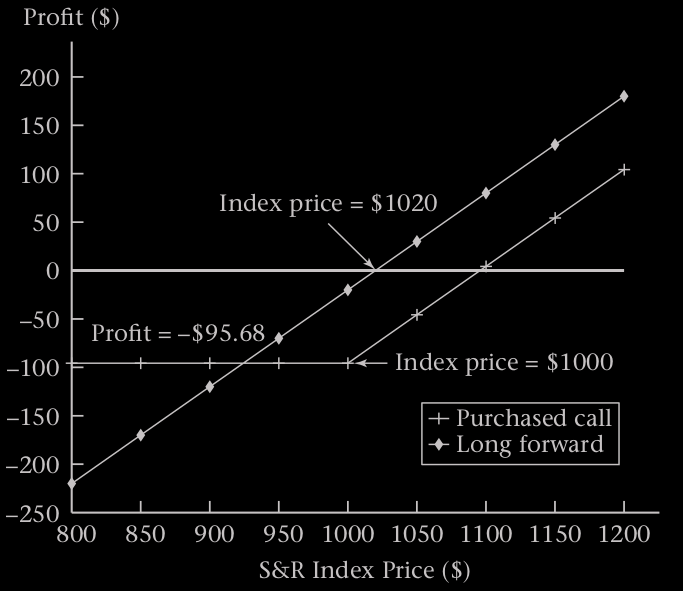
\includegraphics[scale=0.2]{figs/Figure-2-6.png}
\end{center}
\end{frame}
%-------------- end slide -------------------------------%}}}
%-------------- start slide -------------------------------%{{{ 1
\begin{frame}[fragile,t]
	\begin{myexample}
		 S\&R Index 6-month European call option
		 \begin{align*}
			 \text{Strike price}           & = \$1,000, \\
			 \text{Premium}                & = \$93.81, \\
			 \text{6-month risk-free rate} & = 2\%.
		 \end{align*}
		 Compute both payoff and profit of the \textcolor{alert}{written} call option if the index
		 value in six months $\textcolor{magenta}{\$1,100}$ (resp.  $\textcolor{cyan}{\$900}$).
	\end{myexample}
	\bigskip
	\pause
	\begin{mysol}\phantom{a}\\[1em]

	 \begin{minipage}{0.48\textwidth}
		\begin{center}
			If index value in six months = \textcolor{magenta}{\$1,100},
			\begin{align*}
				\text{Payoff} & = - \max ( 0, \textcolor{magenta}{\$1,100} – \$1,000 ) \\
                      & = - \$100                                              \\
				\text{Profit} & = - \$100 + \$93.81 \times 1.02                        \\
                      & = - \$4.32.
			\end{align*}
		\end{center}
	 \end{minipage}
	 \hfill \pause
	 \begin{minipage}{0.48\textwidth}
		\begin{center}
			If index value in six months = \textcolor{cyan}{\$900},
			\begin{align*}
				\text{Payoff} & = - \max ( 0, \textcolor{cyan}{\$900} – \$1,000 ) \\
                      & = \$0                                             \\
				\text{Profit} & = \$0 + \$93.81 \times 1.02                       \\
                      & = \$95.68.
			\end{align*}
		\end{center}
	 \end{minipage}

	 \myEnd
	\end{mysol}
\end{frame}
%-------------- end slide -------------------------------%}}}
%-------------- start slide -------------------------------%{{{ 1
\begin{frame}[fragile]
\begin{center}
	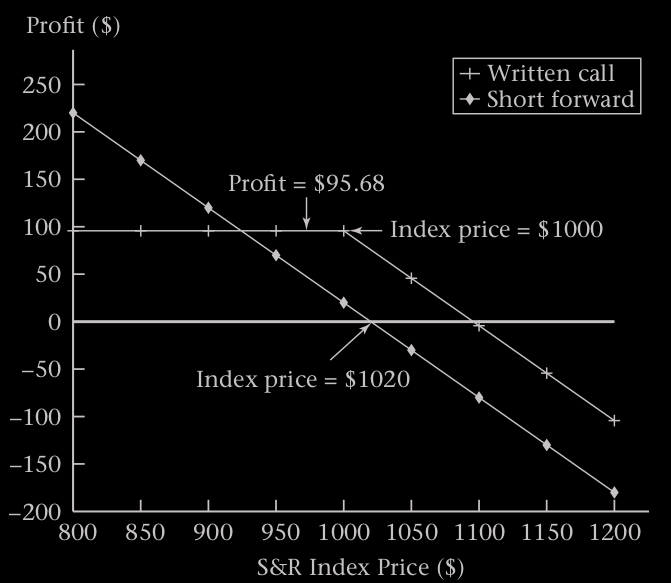
\includegraphics[scale=0.2]{figs/Figure-2-7.png}
\end{center}
\end{frame}
%-------------- end slide -------------------------------%}}}


\def\mySecNum{2.3}
\mySection{\mySecNum~Put options}
%-------------- start slide -------------------------------%{{{ 1
\begin{frame}[fragile]
	\begin{center}
		Call option	: \textcolor{magenta}{Buyer} can walk away.

		\bigskip
		\mySeparateLine
		\bigskip

		???? option : \textcolor{cyan}{Seller} can walk away.
	\end{center}
\end{frame}
%-------------- end slide -------------------------------%}}}
%-------------- start slide -------------------------------%{{{ 1
\begin{frame}[fragile,t]

	\begin{mydefinition}
		A \textcolor{magenta}{put option} gives the owner the right but not the obligation to sell the
		underlying asset at a predetermined price during a predetermined time period.
	\end{mydefinition}
	\bigskip

	\begin{remark}
		Similar to the call option case, a premium paid by the put buyer at the time the option is
		purchased is needed in order to compensate the put seller for being in a disadvantage position.
	\end{remark}
	\bigskip

	\begin{center}
		\renewcommand{\arraystretch}{1.2}
		\begin{tabular}{|c|c|cc|}
			\hline
			... of put option & someone needs to &                     & premium \\ \hline
			seller            & buy              & has to buy if asked & receive \\
			buyer             & sell             & can walk away       & pay     \\
			\hline
		\end{tabular}
	\end{center}
\end{frame}
%-------------- end slide -------------------------------%}}}
%-------------- start slide -------------------------------%{{{ 1
\begin{frame}[fragile,t]
	\begin{align*}
		\text{\textcolor{magenta}{Payoff} of purchased put} & = \max \left( 0,  \text{strike price} - \text{spot price at expiration}\right) \\[1em]
		\text{\textcolor{cyan}{Profit} of purchased put}    & = \text{\textcolor{magenta}{payoff} of purchased put}                          \\
                                                        & \quad -\text{future value of option premium}
	\end{align*}
	\bigskip
	\mySeparateLine
	\bigskip
	\begin{align*}
		\text{\textcolor{magenta}{Payoff} of written put} & = - \max \left( 0,  \text{strike price} - \text{spot price at expiration} \right) \\[1em]
		\text{\textcolor{cyan}{Profit} of written put}    & = \text{\textcolor{magenta}{payoff} of written put}                               \\
                                                      & \quad + \text{future value of option premium}
	\end{align*}
\end{frame}
%-------------- end slide -------------------------------%}}}
%-------------- start slide -------------------------------%{{{ 1
\begin{frame}[fragile,t]
	\begin{myexample}
		 S\&R Index 6-month European put option
		 \begin{align*}
			 \text{Strike price}           & = \$1,000, \\
			 \text{Premium}                & = \$74.20, \\
			 \text{6-month risk-free rate} & = 2\%.
		 \end{align*}
		 Compute both payoff and profit of the \textcolor{alert}{purchased} put option if the index
		 value in six months $\textcolor{magenta}{\$1,100}$ (resp.  $\textcolor{cyan}{\$900}$).
	\end{myexample}
	\bigskip
	\pause
	\begin{mysol}\phantom{a}\\[1em]

	 \begin{minipage}{0.48\textwidth}
		\begin{center}
			If index value in six months = \textcolor{magenta}{\$1,100},
			\begin{align*}
				\text{Payoff} & = \max ( 0, \$1,000 - \textcolor{magenta}{\$1,100}) \\
                      & = \$0                                               \\
				\text{Profit} & = \$0 - \$74.20 \times 1.02                         \\
                      & = - \$75.68.
			\end{align*}
		\end{center}
	 \end{minipage}
	 \hfill \pause
	 \begin{minipage}{0.48\textwidth}
		\begin{center}
			If index value in six months = \textcolor{cyan}{\$900},
			\begin{align*}
				\text{Payoff} & = \max ( 0, \$1,000 - \textcolor{cyan}{\$900} ) \\
                      & = \$100                                           \\
				\text{Profit} & = \$100 - \$74.20 \times 1.02                     \\
                      & = \$24.32.
			\end{align*}
		\end{center}
	 \end{minipage}

	 \myEnd
	\end{mysol}
\end{frame}
%-------------- end slide -------------------------------%}}}
%-------------- start slide -------------------------------%{{{ 1
\begin{frame}[fragile]
\begin{center}
	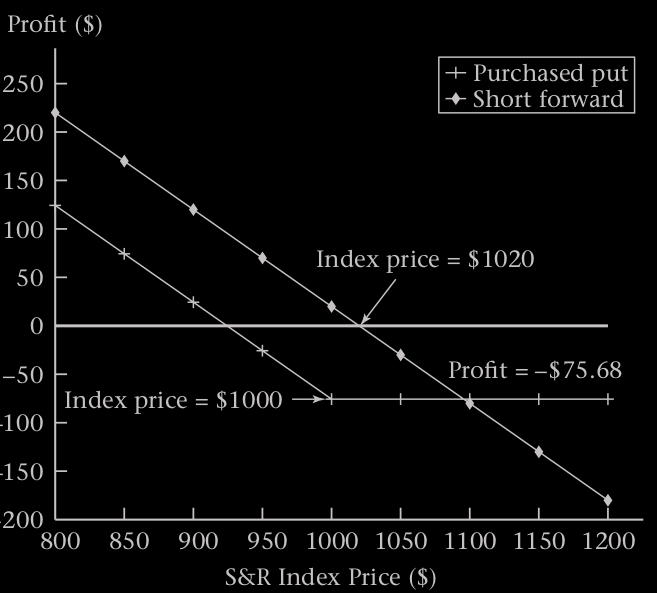
\includegraphics[scale=0.2]{figs/Figure-2-8.png}
\end{center}
\end{frame}
%-------------- end slide -------------------------------%}}}
%-------------- start slide -------------------------------%{{{ 1
\begin{frame}[fragile,t]
	\begin{myexample}
		 S\&R Index 6-month European put option
		 \begin{align*}
			 \text{Strike price}           & = \$1,000, \\
			 \text{Premium}                & = \$74.20, \\
			 \text{6-month risk-free rate} & = 2\%.
		 \end{align*}
		 Compute both payoff and profit of the \textcolor{alert}{written} put option if the index
		 value in six months $\textcolor{magenta}{\$1,100}$ (resp.  $\textcolor{cyan}{\$900}$).
	\end{myexample}
	\bigskip
	\pause
	\begin{mysol}\phantom{a}\\[1em]

	 \begin{minipage}{0.48\textwidth}
		\begin{center}
			If index value in six months = \textcolor{magenta}{\$1,100},
			\begin{align*}
				\text{Payoff} & = - \max ( 0, \$1,000 - \textcolor{magenta}{\$1,100}) \\
                      & = \$0                                                 \\
				\text{Profit} & = \$0 + \$74.20 \times 1.02                           \\
                      & = \$75.68.
			\end{align*}
		\end{center}
	 \end{minipage}
	 \hfill \pause
	 \begin{minipage}{0.48\textwidth}
		\begin{center}
			If index value in six months = \textcolor{cyan}{\$900},
			\begin{align*}
				\text{Payoff} & = - \max ( 0, \$1,000 - \textcolor{cyan}{\$900} ) \\
                      & = - \$100                                         \\
				\text{Profit} & = - \$100 + \$74.20 \times 1.02                   \\
                      & = - \$24.32.
			\end{align*}
		\end{center}
	 \end{minipage}

	 \myEnd
	\end{mysol}
\end{frame}
%-------------- end slide -------------------------------%}}}
%-------------- start slide -------------------------------%{{{ 1
\begin{frame}[fragile]
\begin{center}
	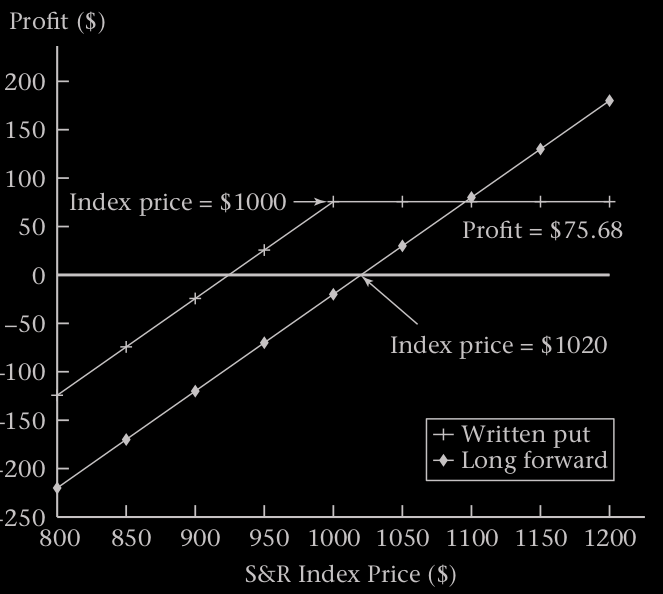
\includegraphics[scale=0.2]{figs/Figure-2-9.png}
\end{center}
\end{frame}
%-------------- end slide -------------------------------%}}}
%-------------- start slide -------------------------------%{{{ 1
\begin{frame}[fragile]
	\begin{center}
		A \textcolor{magenta}{call} option becomes more profitable \\
		when the underlying asset                                  \\
		\textcolor{magenta}{appreciates} in value

		\bigskip
		\mySeparateLine
		\bigskip

		A \textcolor{cyan}{put} option becomes more profitable     \\
		when the underlying asset                                  \\
		\textcolor{cyan}{depreciates} in value
	\end{center}
\end{frame}
%-------------- end slide -------------------------------%}}}
%-------------- start slide -------------------------------%{{{ 1
\begin{frame}[fragile,t]
	\begin{mydefinition}
		\textcolor{magenta}{Moneyness} of an option describes whether the option payoff would be
		positive if the option were exercised immediately.
		\bigskip

		In particular, one has
		\bigskip

		\begin{center}
			\renewcommand{\arraystretch}{1.2}
			\begin{tabular}{|c|c|}
				\hline
				Moneyness                                    & payoff if exercised immediately \\ \hline
				\textcolor{magenta}{In-the-money option}     & $>0$                            \\
				\textcolor{magenta}{At-the-money option}     & $=0$                            \\
				\textcolor{magenta}{Out-of-the money option} & $<0$                            \\ \hline
			\end{tabular}
		\end{center}
	\end{mydefinition}
\end{frame}
%-------------- end slide -------------------------------%}}}

\def\mySecNum{2.4}
\mySection{\mySecNum~Options are insurance}
%-------------- start slide -------------------------------%{{{ 1
\begin{frame}[fragile,t]
\begin{myexample}
  Homeowner's insurance is a put option:
\begin{align*}
	\text{Value of house} & = \$200,000 \\
	\text{Deductible}     & = \$25,000  \\
	\text{Premium}        & = \$15,000
\end{align*}
\end{myexample}
\begin{center}
	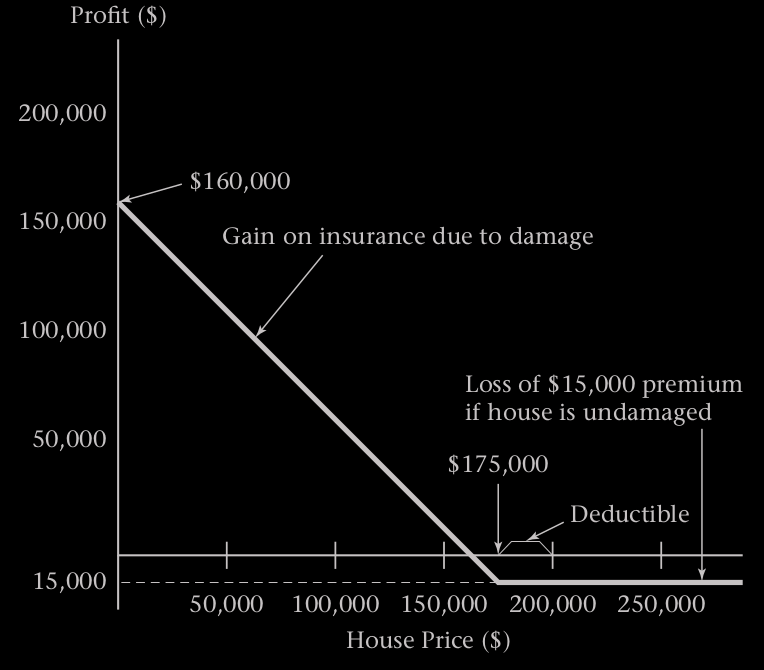
\includegraphics[scale=0.22]{figs/Figure-2-12.png}
\end{center}
\end{frame}
%-------------- end slide -------------------------------%}}}
%-------------- start slide -------------------------------%{{{ 1
\begin{frame}[fragile]
\begin{center}
	\begin{minipage}{0.5\textwidth}
		\centering
		The premium of the insurance \\
		or                           \\
		the value of the put option  \\
		depends on\\

		\begin{itemize}
			\item Riskiness of the underlying asset
			\item The amount of deductible.
		\end{itemize}
	\end{minipage}

	\pause
	\bigskip
	\mySeparateLine
	\bigskip

	\begin{minipage}{0.65\textwidth}
		\centering
		Difference with options

		\begin{itemize}
			\item Put option pays off no matter why the index price declines.
			\item Insurance pays off only if the house declines in value for for specific reasons.
		\end{itemize}
	\end{minipage}

\end{center}
\end{frame}
%-------------- end slide -------------------------------%}}}
%-------------- start slide -------------------------------%{{{ 1
\begin{frame}[fragile]
	\begin{center}

		\begin{minipage}{0.5\textwidth}
			\centering

			A \textcolor{magenta}{put} option is \\
			\alert{an insurance}                 \\

			\begin{enumerate}
				\item for an asset we already own.
				\item for a long position.
				\item against an decrease in value.
			\end{enumerate}
		\end{minipage}

		\pause
		\bigskip
		\mySeparateLine
		\bigskip

		\begin{minipage}{0.5\textwidth}
			\centering

			A \textcolor{cyan}{call} option is \\
			\alert{an insurance}               \\

			\begin{enumerate}
				\item for an asset we plan to own in the future.
				\item for a short position.
				\item against an increase in price.
			\end{enumerate}
		\end{minipage}
	\end{center}

\end{frame}
%-------------- end slide -------------------------------%}}}

\def\mySecNum{2.5}
\mySection{\mySecNum~Summary of forward and option positions}
%-------------- start slide -------------------------------%{{{ 1
\begin{frame}[fragile]
\begin{eqnarray*}
	\left\{\text{long},\text{short}\right\} & \times & \left\{\text{forward}, \text{call}, \text{put}\right\} \\[1.2em]
                                          & |  |   &
\end{eqnarray*}
\begin{align*}
	\text{six positions}\hspace{3em}
\end{align*}
\end{frame}
%-------------- end slide -------------------------------%}}}
%-------------- start slide -------------------------------%{{{ 1
\begin{frame}[fragile,t]

\begin{center}
	Maximum possible profit and loss at maturity for \\
	$\left\{\text{long},\text{short}\right\} \times \left\{\text{forward}, \text{call}, \text{put}\right\}$
	\mySeparateLine
	\bigskip

	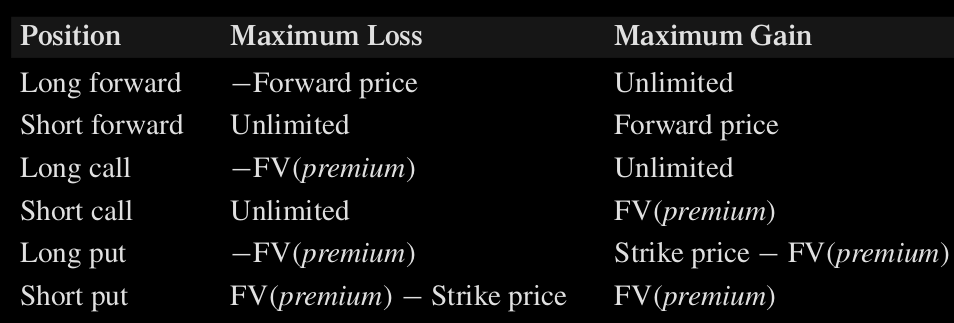
\includegraphics[scale=0.3]{figs/Table2-5.png}\footnote{$FV(\cdot)$ denotes the function that returns the future value.}
\end{center}
\end{frame}
%-------------- end slide -------------------------------%}}}
%-------------- start slide -------------------------------%{{{ 1
\begin{frame}[fragile]
\begin{center}
	Profit diagrams for \\
	$\left\{\text{long},\text{short}\right\} \times \left\{\text{forward}, \text{call}, \text{put}\right\}$
	\mySeparateLine
	\bigskip

	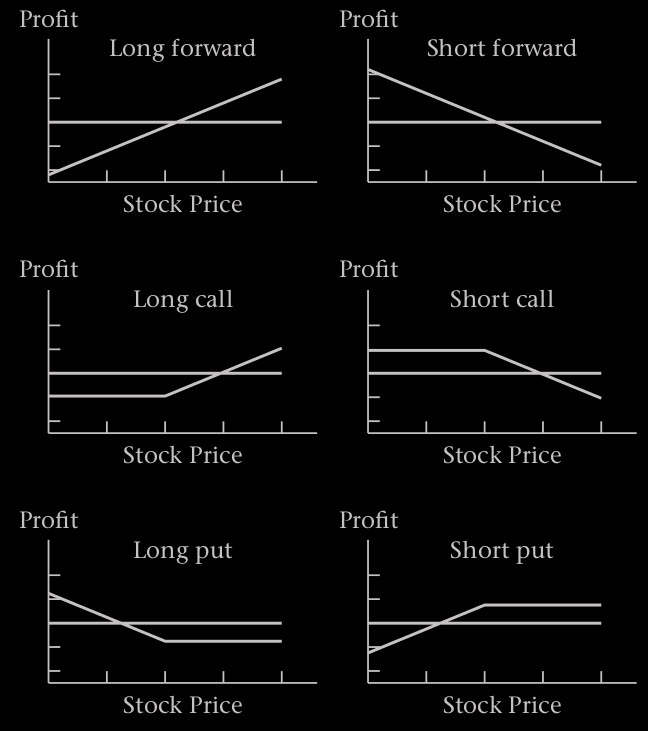
\includegraphics[scale=0.27]{figs/Figure-2-14.png}
\end{center}
\end{frame}
%-------------- end slide -------------------------------%}}}
%-------------- start slide -------------------------------%{{{ 1
\begin{frame}[fragile]
\begin{center}
	Summary of positions for \\
	$\left\{\text{long},\text{short}\right\} \times \left\{\text{forward}, \text{call}, \text{put}\right\}$
	\mySeparateLine
	\bigskip

	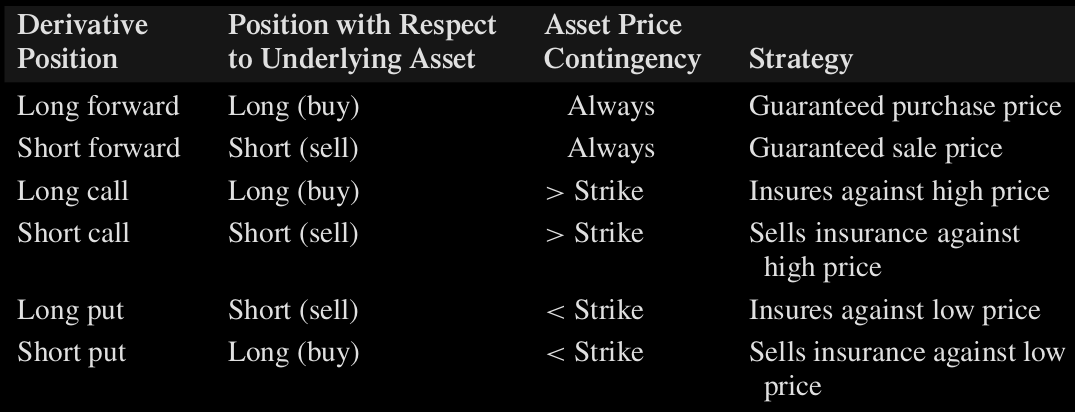
\includegraphics[scale=0.25]{figs/Table-2-7.png}
\end{center}
\end{frame}
%-------------- end slide -------------------------------%}}}

\def\mySecNum{2.6}
\mySection{\mySecNum~Problems}
%-------------- start slide -------------------------------%{{{ 1
\begin{frame}[fragile,t]
	Problems:
	2.1,
	2.2,
	2.4,
	2.5,
	2.6,
	2.7,
	2.8,
	2.9,
	2.13,
	2.14.
	\\
	\bigskip

	Due Date: TBA
\end{frame}
%-------------- end slide -------------------------------%}}}

\end{document}
